\chapter{Forces and Frames}
\begin{marginfigure}%
  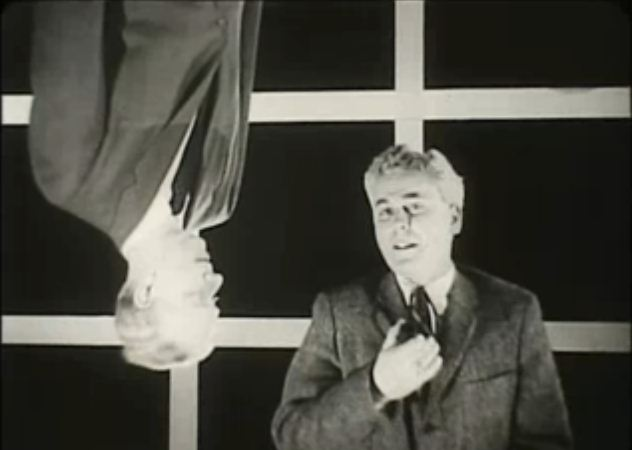
\includegraphics[width=\linewidth]{Frames.jpg}
  \caption{Frames of Reference is a 1960 educational film by Physical Sciences Study Committee.}
  \label{fig:marginfig}
\end{marginfigure}
\textit{The people... are the motive force.}  \\
\noindent\textbf{-  Mao Tse Tung}
\vspace{1cm}
\marginnote[30pt]{An inertial frame of reference is in a state of constant, rectilinear motion.  It is peaceful and non-accelerating.  Inertial is synonymous  with Newtonian and Galilean.  Newton's laws are only applicable in an inertial frame of reference.}


\section{Principia}
\textit{Philosophi\ae \ Naturalis Principia Mathematica}, Latin for "Mathematical Principles of Natural Philosophy", is often referred to simply as the Principia.  The work consists of three books by Sir Isaac Newton, in Latin, first published in 1687.  The Principia states Newton's laws of motion, forming the foundation of classical mechanics, also Newton's law of universal gravitation, and a mathematical derivation of Kepler's empirically derived laws of planetary motion. The Principia is justly regarded as one of the most important works in the history of science.

\begin{marginfigure}[30pt]%
  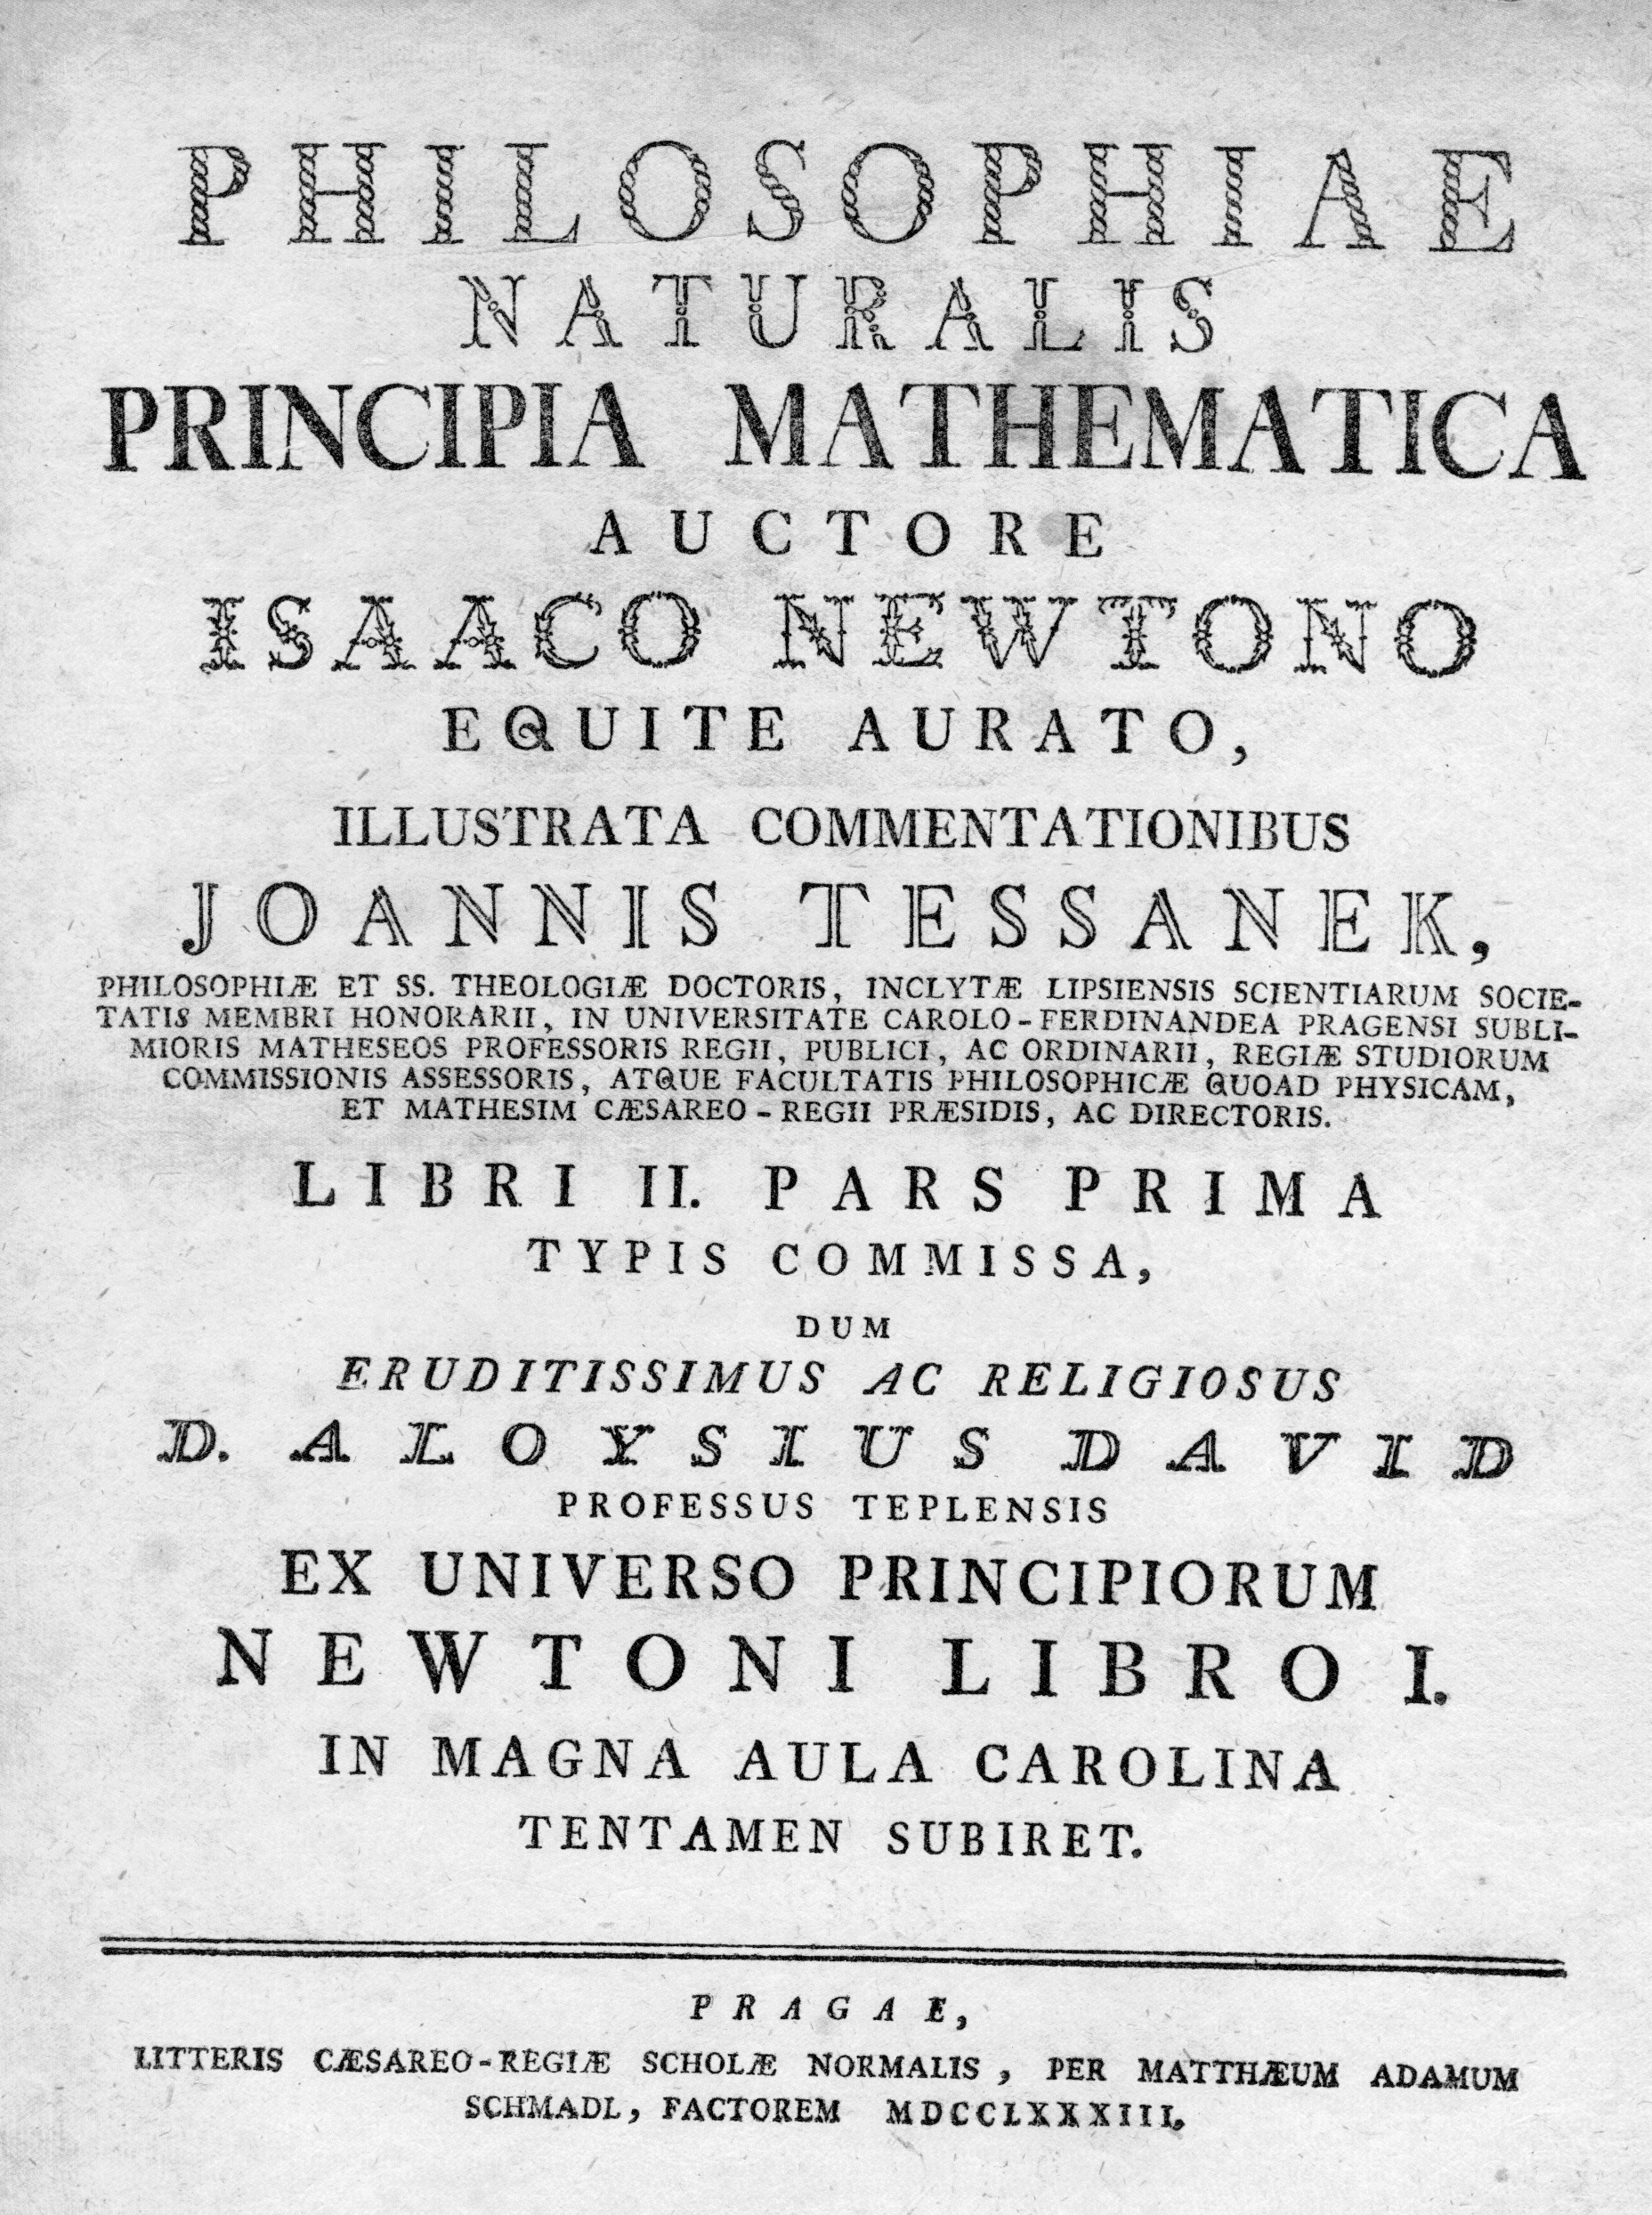
\includegraphics[width=\linewidth]{principia.jpg}
  \caption{The Principia}
  \label{fig:marginfig}
\end{marginfigure}


\section{Newton's First Law}


\textit{Every body perseveres in its state of being at rest or of moving uniformly straight forward, except insofar as it is compelled to change its state by forces impressed.} \textbf{\textit{- Principia}}


$$\sum \overrightarrow{F}=0\ \ \longrightarrow \ \ \overrightarrow{a}=0$$

\newthought{In an inertial frame}, an object at rest tends to stay at rest and an object in motion tends to stay in motion unless an external net force acts upon it.  Newton's first law is often called the Law of Inertia.

\newpage

 \marginnote[50pt]{
\textit{Inherent force of matter is the power of resisting by which every body, so far as it is able, perseveres in its state either of resting or of moving uniformly straight forward.}\\   \noindent\textbf{\textit{- Principia}}}
\subsection{Inertia}
\newthought{Inertia is the resistance} of any physical object to any change in its state of motion including changes to its speed and direction or the state of rest. It is the tendency of objects to keep moving in a straight line at constant velocity. The principle of inertia is one of the fundamental principles of classical physics that are used to describe the motion of objects and how they are affected by applied forces. Inertia comes from the Latin word, iners, meaning idle, sluggish. Inertia is one of the primary manifestations of mass.  Matter is the occupancy of mass over space therefore matter has inertia.
 


\begin{marginfigure}[110pt]%
  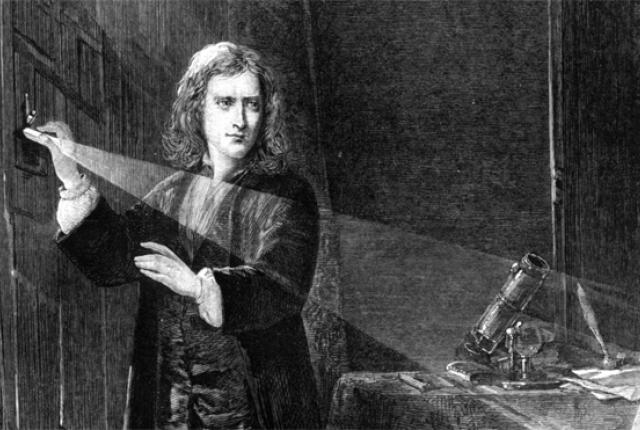
\includegraphics[width=\linewidth]{isaac-newton.jpg}
  \caption{Isaac Newton doing his thing}
  \label{fig:marginfig}
\end{marginfigure}
 
\subsection{  Space and Time Uniformity}
\begin{description}
  \item [Homogeneity] A homogeneous system has the same properties at every point; it is uniform without irregularities.  The laws of physics must be invariant (unchanging) to translations in space.  The location of the coordinate system does not change physics.
  \item [Isotropy]  A isotropic system has the same properties in all directions.  The laws of physics must be invariant to rotations in space.  The orientation of the coordinate system does not change physics.  
  \item [Time-Independence] A time-independent system has the same properties throughout time.  The laws of physics must be invariant to translations in time.  The start time of the physicist's watch does not change physics.
 \end{description}








\section{Newton's Second Law}
\marginnote[0pt]{
\textit{A change in motion is proportional to the motive force impressed and takes place along the straight line in which that force is impressed.}  \\   \noindent\textbf{\textit{- Principia}}
}

Newton's second law states the sum of forces on an object is equal to the product of mass and acceleration of the object.
$$F_{net}=ma$$

Stated another way, the sum of forces is equal to the time rate of change of momentum.

$$\sum \overrightarrow{F}=\lim_{\Delta \rightarrow 0}\frac{\Delta \overrightarrow{p}}{\Delta t}=\lim_{\Delta \rightarrow 0}\frac{\Delta (m\overrightarrow{v})}{\Delta t}=m\lim_{\Delta \rightarrow 0}\frac{\Delta \overrightarrow{v}}{\Delta t}=m\overrightarrow{a}$$

\newthought{Momentum is defined} as the product of mass and velocity. Though Newton does not use the term he describes a \textit{quantitas motus}, "quantity of motion", as "arising from the velocity and quantity of matter conjointly", which identifies it as momentum.  Thus, in the second law, when he refers to \textit{mutatio motus} being proportional to the force impressed, he is generally taken to mean momentum again.  It remained only to assign a standard term to the quantity of motion. The first use of "momentum" in its proper mathematical sense is not known but Jenning's 1721 \textit{Miscellanea} defines momentum, or "quantity of motion", as "a rectangle", the product of Q and V, where Q is "quantity of material" and V is "velocity".  

\marginnote[-80pt]{
\textit{The quantity of matter is that which arises conjointly from its density and magnitude. A body twice as dense in double the space is quadruple in quantity. This quantity I designate by the name of body or of mass.}
\\   \noindent\textbf{\textit{- Principia}}
}
$$\underbrace{\overrightarrow{p}}_{\textit{momentum}}=\overbrace{m}^{\textit{inertial mass}}\underbrace{\overrightarrow{v}}_{\textit{velocity}}$$

\begin{marginfigure}[40pt]%
  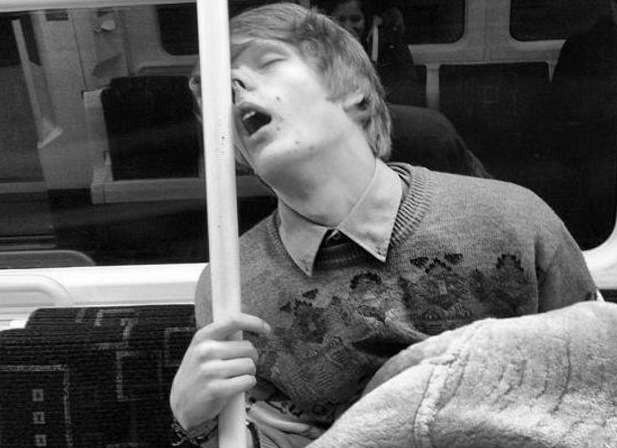
\includegraphics[width=\linewidth]{snore.jpg}
  \caption{If you wakeup from sleeping on a train moving at constant velocity, there is nothing about the physics in the train that tells you it's moving.  The constant velocity train is inertial and a legit frame of reference from which to do physics.}
  \label{fig:marginfig}
\end{marginfigure}
\newthought{Galilean invariance} or Galilean relativity states that the laws of motion are the same in all inertial frames. Galileo Galilei first described this principle in 1632 in his Dialogue Concerning the Two Chief World Systems using the example of a ship travelling at constant velocity, without rocking, on a smooth sea; any observer doing experiments below the deck would not be able to tell whether the ship was moving or stationary.  Newton's second law is invariant to change in the velocity of the frame.


\section{Newton's Third Law}
\newthought{The third law states} that all forces between two objects exist in equal magnitude and opposite direction: if object one exerts a force $\overrightarrow{F}_{ 1\rightarrow 2}$ on object two , then object two simultaneously exerts a force $\overrightarrow{F}_{ 2\rightarrow 1}$ on object one, and the two forces are equal in magnitude but opposite in direction.
$$\overrightarrow{F}_{ 1\rightarrow 2}=-\overrightarrow{F}_{2\rightarrow 1}$$

The third law means that all forces are interactions between different bodies,and thus that there is no such thing as a unidirectional force or a force that acts on only one body. This law is sometimes referred to as the action-reaction law, with $\overrightarrow{F}_{ 1\rightarrow 2}$ called the "action" and $\overrightarrow{F}_{ 2\rightarrow 1}$ the "reaction". The action and the reaction are simultaneous, and it does not matter which is called the action and which is called reaction; both forces are part of a single interaction, and neither force exists without the other.

\marginnote[-130pt]{\textit{To any action there is always an opposite and equal reaction; in other words, the actions of two bodies upon each other are always equal and always opposite in direction. }\\   \noindent\textbf{\textit{- Principia}}
}

\newthought{The contemporary mantra} for Newton's third law is uttered as follows.\\ \ \\ \textbf{Every action has an equal and opposite reaction.}

\begin{marginfigure}[-40pt]%
  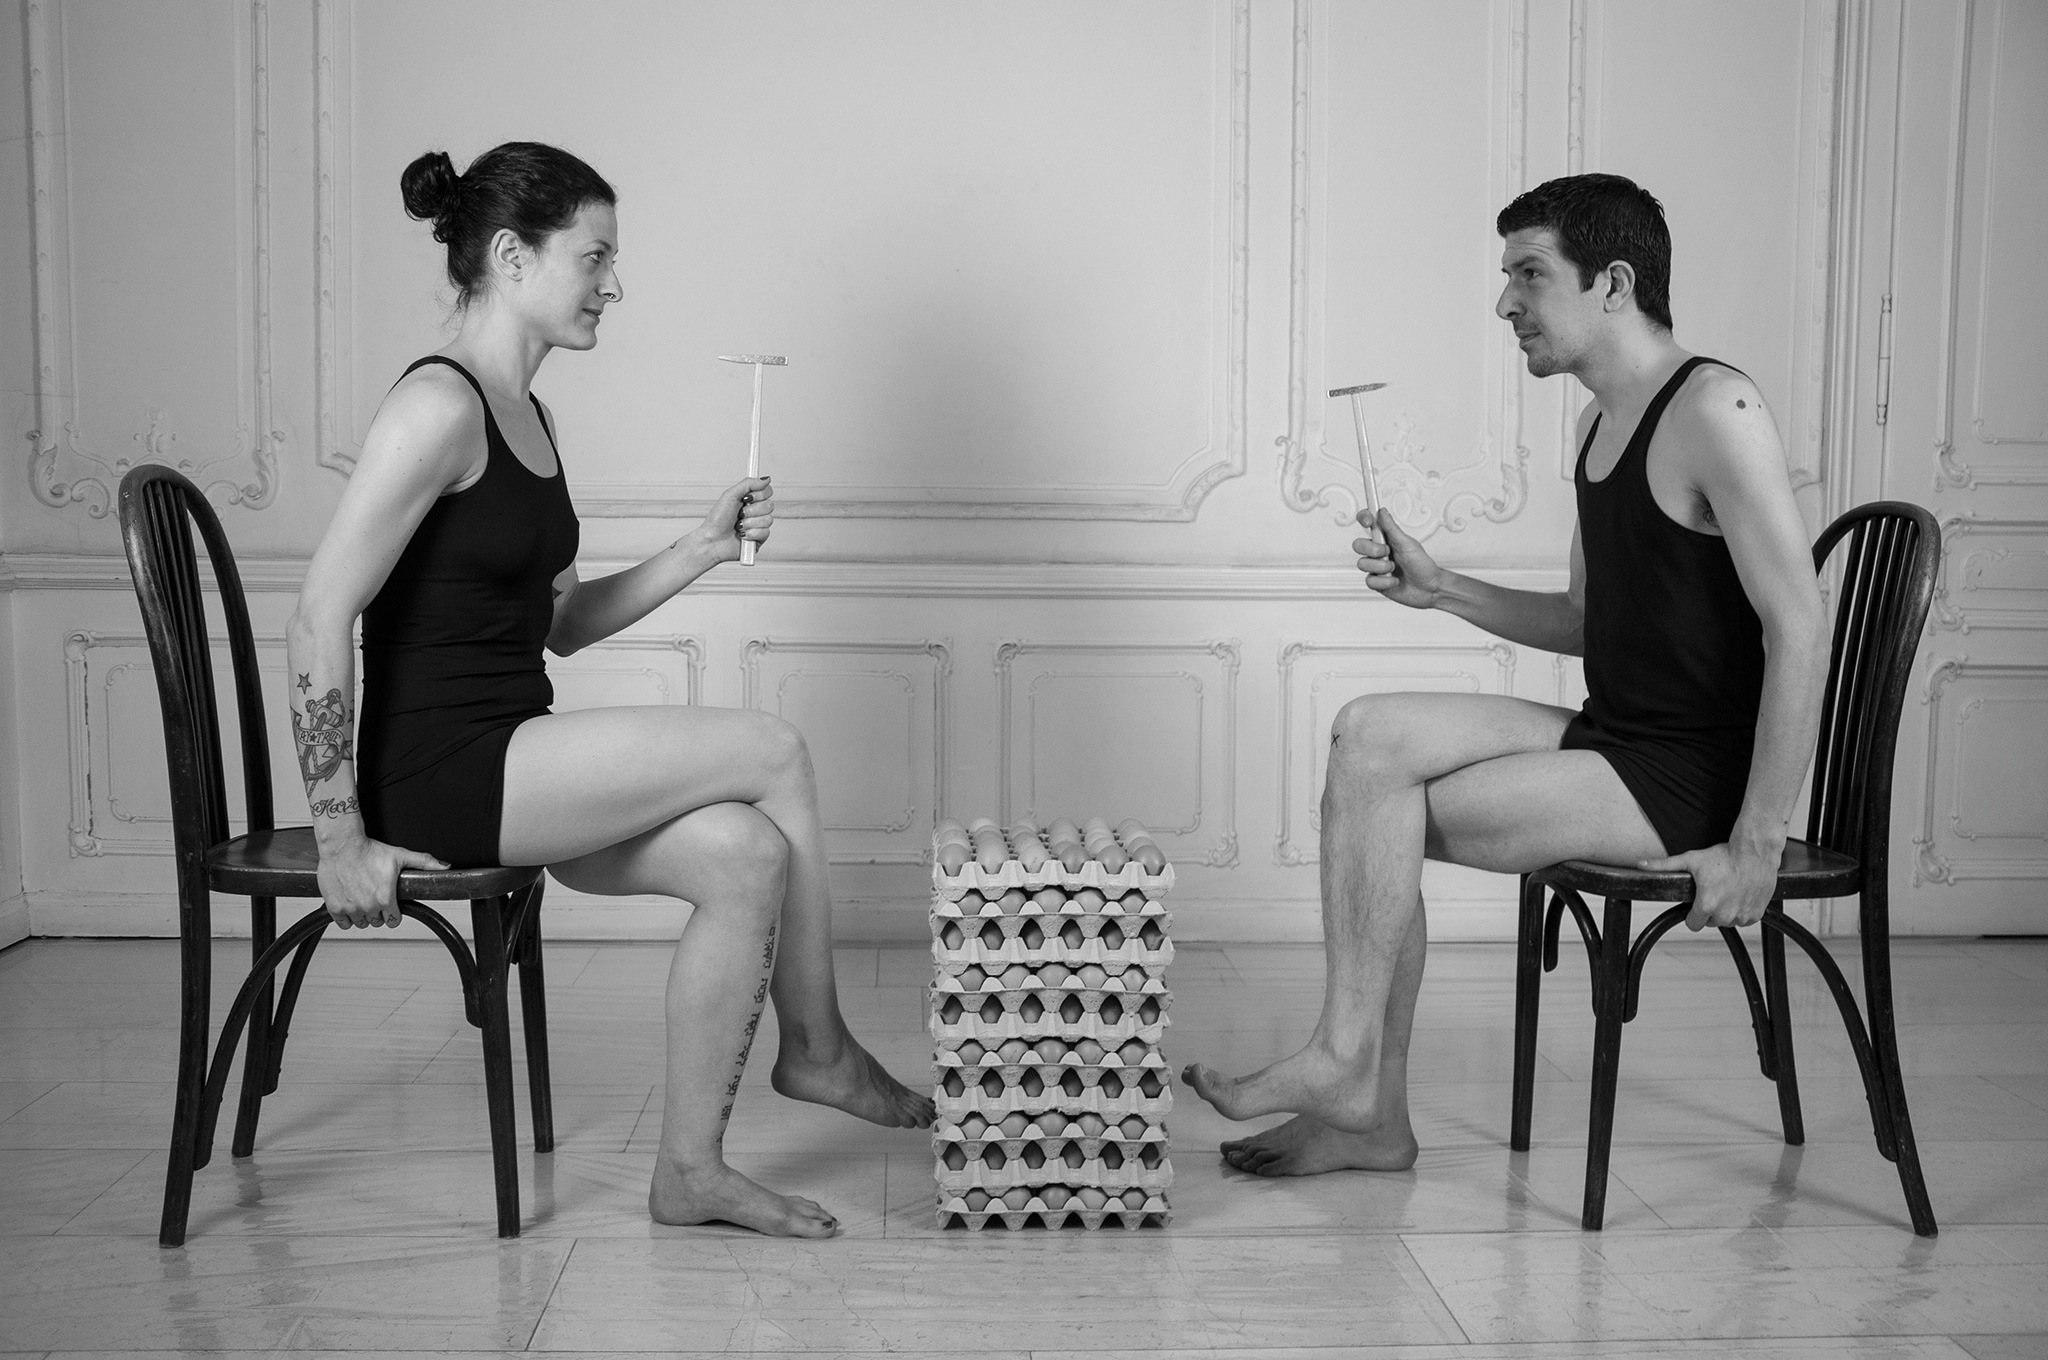
\includegraphics[width=\linewidth]{reaction.jpg}
  \caption{Action/Reaction was a 2014 performance art work by Rahman Hak-Hagir and Francesca Lolli.}
  \label{fig:marginfig}
\end{marginfigure}


\newpage

\section{Forces}
Forces are vector quantities as they had magnitudes and direction in space.  Summation of forces follows vector addition.   The unit of force is the Newton, or N.  This is one kilogram meter per square second.  

\marginnote[-40pt]{The English pound is a unit of force equivalent to $4.45$ Newtons.
$$1\ \text{lbs}=4.45\ \text{N}$$}

$$1\ \text{Newton}=\frac{\text{kg}\cdot\text{m}}{\text{s}^2}$$



\subsection{Statics}
\newthought{Statics is the branch of mechanics} that is concerned with the analysis of force loads on physical systems in static equilibrium, that is, in an inertial state where the relative positions of subsystems do not vary over time.  When in static equilibrium, the system is not being accelerated.  Therefore, by Newton's first law, the vector sum of the forces is zero.

\begin{marginfigure}[-50pt]%
  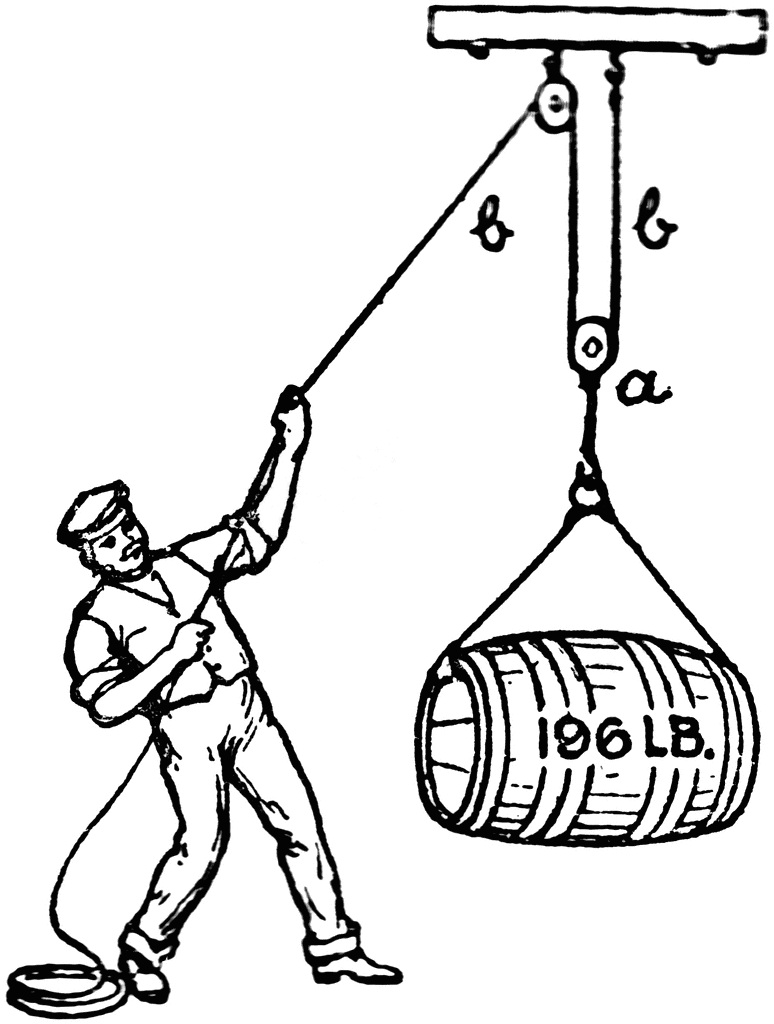
\includegraphics[width=\linewidth]{pulley.jpg}
  \caption{This could be a static or dynamic system, depending on the balance of forces.}
  \label{fig:marginfig}
\end{marginfigure}

\subsection{Dynamics} 
\newthought{Dynamics is the branch of mechanics} concerned with the study of forces and and their effect on motion.  In a dynamic situation the net force is non-zero and there is a resultant acceleration.  Newton's second law is invoked when analyzing a dynamic system. 



\section{Free Body Diagrams}
\newthought{A free body diagram is a graphical illustration} used to visualize and conceive of the applied forces on a body.  In the current treatment we represent particles with a dot and draw all forces incident on the particle as a vector diagram with all force vectors with their tail at the point.  

\marginnote[-70pt]{Once a coordinate system is established all forces can be decomposed in terms of components and summed across the component directions.  The resultant force determines the acceleration.  In some cases first knowing the acceleration gives an understanding of the constituent forces. }


\begin{fullwidth}
\vspace{0.5cm}
$$\overrightarrow{F}_{net}=\overrightarrow{F}_1+\overrightarrow{F}_2=\left(\begin{array}{c} \overrightarrow{F}_{2,x}  \\ \overrightarrow{F}_{1,y} +\overrightarrow{F}_{2,y}  \end{array}\right)=m\overrightarrow{a}\ \ \Longrightarrow \ \ \overrightarrow{a}=\frac{1}{m}\left(\begin{array}{c} \overrightarrow{F}_{2,x}  \\ \overrightarrow{F}_{1,y} +\overrightarrow{F}_{2,y}  \end{array}\right)$$
\vspace{0.5cm}
$$\begin{tikzpicture}[scale=1]
   	\draw[->,thick] (0,0) -- (0,-1) node [anchor=north ,scale=1] {$F_1 $}; 
     	\draw[->,thick] (0,0) -- ({2^0.5},{2^0.5}) node [anchor=south ,scale=1] {$F_2 $}; 
    	\fill[black] (0,0) circle (0.5mm);
    
     \begin{scope}[shift={(3,0.2)}, scale=0.75]
	  \draw[ thick,-stealth] (0,-0.1) -- (0,0.8) node [near start,anchor=east]{\scriptsize $y$};  
	  \draw[thick](-0.1,0) -- (0.1,0);
	   \draw[thick](0.2,-0.4) -- (0.2,-0.6);
	    \draw[ thick,-stealth] (0.1,-0.5) -- (1,-0.5) node [near start,anchor=north]{\scriptsize $x$};  
   \end{scope}

    
   \begin{scope}[shift={(5,0)}]
    	\draw[->,thick] (0,0) -- (0,-1) node [anchor=north ,scale=1] {$F_{1,y} $}; 
   	\draw[->,thick] (0,0) -- ({2^0.5},{0}) node [anchor=south ,scale=1] {$F_{2,x} $}; 
   	\draw[->,thick] (0,0) -- ({0},{2^0.5}) node [anchor=south ,scale=1] {$F_{2,y} $}; 
   	 \fill[black] (0,0) circle (0.5mm);
   \end{scope}
   
    \begin{scope}[shift={(8,0)}]   
   	  \draw[->,thick] (0,0) -- ({2^0.5 },{0}) node [anchor=south ,scale=1] {$F_{net,x} $}; 
   	   \draw[->,thick] (0,0) -- ({0},{2^0.5-1}) node [anchor=south ,scale=1] {$F_{net,y} $}; 
   	 \fill[black] (0,0) circle (0.5mm);
   \end{scope}
   
    \begin{scope}[shift={(11,0)}]
     	\draw[->,thick] (0,0) -- ({2^0.5 },{2^0.5-1}) node [anchor=south ,scale=1] {$F_{net} $};   
   	 \fill[black] (0,0) circle (0.5mm);
   \end{scope}
   
   \end{tikzpicture}
   $$
   \end{fullwidth}
\vspace{0.5cm}
\section{Weight}
\marginnote[30pt]{Modern work on gravitational theory began with the work of Galileo Galilei in the late 16th and early 17th centuries. In his famous (though possibly apocrypha) experiment dropping balls from the Tower of Pisa, and later with careful measurements of balls rolling down inclines, Galileo showed that gravity accelerates all objects at the same rate. This was a major departure from Aristotle's belief that heavier objects accelerate faster. Galileo postulated air resistance as the reason that lighter objects may fall more slowly in an atmosphere. Galileo's work set the stage for the formulation of Newton's theory of gravity.}
\newthought{Gravity is a natural phenomenon} by which all things with mass are brought towards (or 'gravitate' towards) one another including stars, planets, galaxies and even light and sub-atomic particles. Gravity is responsible for the complexity in the universe, by creating spheres of hydrogen, igniting them under pressure to form stars and grouping them into galaxies. Without gravity, the universe would be an uncomplicated one, existing without thermal energy and composed only of equally spaced particles. On Earth, gravity gives weight to physical objects and causes the tides. Gravity has an infinite range, and it cannot be absorbed, transformed, or shielded against.

\marginnote[60pt]{\textbf{Weight is the gravity force on a body.}}

Up until now mass has only been considered in its inertial properties.  Gravity is another feature of mass.  At the surface of the Earth, massive objects accelerate at a rate of $g=9.81\frac{\text{m}}{\text{s}^2}$.  Therefore by Newton's second law it follows that, at the surface of the Earth, the force due to gravity, otherwise known as the \textbf{weight}, is equal to $mg$.
\vspace{1cm}
\section{Constant Weight and Acceleration}
\marginnote[10pt]{The constant $g$ is the magnitude of acceleration due to gravity at the surface of the earth.  The direction of the acceleration is toward the center of the earth, namely down. }
$$g=9.81 \frac{\text{m}}{\text{s}^2}$$
\marginnote[20pt]{The force of gravity, or weight, is notated $\overrightarrow{F}_g$.}
$$F_g=mg$$
\vspace{0.5cm}
$$\overrightarrow{F}_{net}=\overrightarrow{F}_{g}=-\overbrace{m}^{\textit{Gravitational Mass}}g \hat{y}=\left(\begin{array}{c} 0 \\ -mg \end{array}\right)=m\overrightarrow{a}$$
\vspace{0.5cm}
$$\begin{tikzpicture}[scale=1]
 \begin{scope}[shift={(-5,0)}, scale=0.5]
\draw[very thick] (-1,-1) -- (-1,1) -- (1,1) -- (1,-1) -- cycle;  
\draw (0,0) node [anchor=center]{$m$};
 \end{scope}
 
  \begin{scope}[shift={(-2.5,-0.2)}, scale=0.75]
	 
	  \draw[ thick,-stealth] (0,-0.1) -- (0,0.8) node [near start,anchor=east]{\scriptsize $y$};  
	  \draw[thick](-0.1,0) -- (0.1,0);
	 
   	
   \end{scope}

     	\draw[->,thick] (0,0) -- (0,{-2^0.5}) node [anchor=north ,scale=1] {$F_g $}; 
    	\fill[black] (0,0) circle (0.5mm);   
   \end{tikzpicture}
   $$
   $$\overrightarrow{a}=\left(\begin{array}{c} 0  \\ -g \end{array}\right)$$
   
\section{Normal Force}
\marginnote[30pt]{The normal force ,$\overrightarrow{F}_n$ is the contact force between an object and a surface.  The direction of the normal force is directly out of the surface.  If there is no surface contact there is no normal force.}
\vspace{0.5cm}
$$\overrightarrow{F}_{net}=\overrightarrow{A}+\overrightarrow{F}_{n}=(F_n-A) \hat{y}=m\overrightarrow{a}$$
\vspace{0.5cm}
$$\begin{tikzpicture}[scale=1]
     	\draw[->,thick] (0,0) -- (0,{-1}) node [anchor=north ,scale=1] {$A$}; 
	\draw[->,thick] (0,0) -- (0,{2^0.5}) node [anchor=south ,scale=1] {$F_n $}; 
    	\fill[black] (0,0) circle (0.5mm);   
	
	  \begin{scope}[shift={(-5,0)}, scale=0.75]
	  \fill[color=gray!30, path fading=south] (-3,-1) -- (2.5,-1) -- (2.5,-2.5) -- (-3,-2.5) ;
	  \draw[very thick] (-3,-1) -- (2.5,-1) node [midway,anchor=north]{\scriptsize surface $\overrightarrow{a}_s$};  
	   \draw[ thick,-stealth] (-2.5,-1) -- (-2.5,-0.25) node [anchor=south]{$\hat{n}$};  
     	\draw[very thick] (-1,-1) -- (-1,1) -- (1,1) -- (1,-1) -- cycle;  
	 
	\draw (0,0) node [anchor=center]{$m$};
   	
   \end{scope}
   
   	  \begin{scope}[shift={(-1,0)}, scale=0.75]
	 
	  \draw[ thick,-stealth] (0,-0.1) -- (0,0.8) node [near start,anchor=east]{\scriptsize $y$};  
	  \draw[thick](-0.1,0) -- (0.1,0);
	 
   	
   \end{scope}
   \end{tikzpicture}
   $$
   \vspace{0.5cm}
   \marginnote[30pt]{As this free body diagram is drawn the normal force exceeds the applied force $\overrightarrow{A}$, therefore the object must be accelerating in the direction of the normal force.  This situation would arise in an upwardly accelerating elevator where the floor exerts a normal force on a passenger in excess of their weight.}
   
   $$\overrightarrow{a}=\frac{F_n-A}{m}\hat{y}$$
   $$F_n=A+ma_y$$
    $$\text{ surface contact requires\ \  }\ \overrightarrow{a}\cdot\hat{n}=\overrightarrow{a}_s\cdot\hat{n} \text{\ \   \   and     \ \ }(\overrightarrow{F}_n\cdot \hat{y})>0$$
     $$\text{for a non-accelerating surface }\ \overrightarrow{a}_s\cdot\hat{n}=0\ \ \ \Longrightarrow\ \ \ F_{net}=0\ \ \text{and}\ \ F_n=A$$
\vspace{0.5cm}

\section{Tension Force}
 \marginnote[30pt]{Tension describes the pulling force exerted by each end of a string, cable, chain, or similar one-dimensional continuous object, or by each end of a rod, truss member, or similar three dimensional object.}
\vspace{0.5cm}For simplicity this system is weightless.  
$$\overrightarrow{F}_{net}=\overrightarrow{T}=\left(\begin{array}{c} T_x \\ T_y \end{array}\right)=\left(\begin{array}{c} T\sin \theta \\ T\cos \theta \end{array}\right)=m\overrightarrow{a}$$
 \marginnote[60pt]{For simplicity this system is weightless.   The tension is drawn with horizontal and vertical components.  This will correspond to horizontal and vertical components of acceleration.}

\vspace{0.5cm}
$$\begin{tikzpicture}[scale=1]
     	
	\draw[->,thick] (0,0) -- (0.5,1.333) node [anchor=south ,scale=1] {$T$}; 
	\draw[dashed] (0,0) -- (0,1.3) node [midway, anchor=south west] {\tiny$\theta$};
    	\fill[black] (0,0) circle (0.5mm);   
	
	 \begin{scope}[shift={(3,0)}, scale=1]
	 \draw[->,thick] (0,0) -- (0,1.333) node [anchor=south ,scale=1] {$T_y$}; 
	 \draw[->,thick] (0,0) -- (0.5,0) node [anchor=west ,scale=1] {$T_x$}; 
	  \end{scope}
	
	
	  \begin{scope}[shift={(-5,-1)}, scale=0.5]
	  \draw[very thick] (0,1) -- (1.5,5); 
	   \draw[dashed] (1.5,5) -- (1.5,1.5) node [midway, anchor=north east] {\small$\theta$};; 
	  \fill[color=gray!30, path fading=north] (-3,5) -- (3,5) -- (3,7) -- (-3,7) ;
	  \draw[very thick] (-3,5) -- (3,5);  
	      	\draw[very thick] (-1,-1) -- (-1,1) -- (1,1) -- (1,-1) -- cycle;  
	 
	\draw (0,0) node [anchor=center]{$m$};
   	
   \end{scope}
   
   
   	  \begin{scope}[shift={(-2,0.2)}, scale=0.75]
	 
	  \draw[ thick,-stealth] (0,-0.1) -- (0,0.8) node [near start,anchor=east]{\scriptsize $y$};  
	  \draw[thick](-0.1,0) -- (0.1,0);
	   \draw[thick](0.2,-0.4) -- (0.2,-0.6);
	    \draw[ thick,-stealth] (0.1,-0.5) -- (1,-0.5) node [near start,anchor=north]{\scriptsize $x$};  
	 
   	
   
   
  
	 
   	
   \end{scope}
   \end{tikzpicture}
   $$
   
 
\newpage
\section{Friction Forces}
\marginnote[10pt]{Friction is the force resisting the relative motion of solid surfaces sliding against each other.  Friction is not itself a fundamental force. Dry friction arises from a combination of inter-surface adhesion, surface roughness, surface deformation, and surface contamination. The complexity of these interactions makes the calculation of friction from first principles impractical and necessitates the use of empirical methods.}
\subsection{Kinetic Friction}
\vspace{0.5cm}
\marginnote[10pt]{Kinetic friction is modeled as a force directly proportional to the normal force and in the opposite direction of sliding.  The constant of proportionality is termed $\mu_k$.}
$$\overrightarrow{F}_{f}=-\mu_kF_n \hat{v}$$
$$\overrightarrow{F}_{net}=\overrightarrow{A}+\overrightarrow{F}_{n}+\overrightarrow{F}_{f}=\left(\begin{array}{c} -F_f \\ F_n-A \end{array}\right)=m\overrightarrow{a}$$
\vspace{0.5cm}
$$\begin{tikzpicture}[scale=1]
     	\draw[->,thick] (0,0) -- (0,-1) node [anchor=north ,scale=1] {$A $}; 
	\draw[->,thick] (0,0) -- (0,1) node [anchor=south ,scale=1] {$F_n $}; 
	\draw[->,thick] (0,0) -- (-0.7,0) node [anchor=east ,scale=1] {$F_f $}; 
    	\fill[black] (0,0) circle (0.5mm);   
	
	  \begin{scope}[shift={(-5,0)}, scale=0.75]
	  \fill[color=gray!30, path fading=south] (-3,-1) -- (2.5,-1) -- (2.5,-2.5) -- (-3,-2.5) ;
	  \draw[very thick] (-3,-1) -- (2.5,-1) node [midway,anchor=north]{\scriptsize surface $\overrightarrow{a}_s=0$};  
	   \draw[ thick,-stealth] (-2.5,-1) -- (-2.5,-0.25) node [anchor=south]{$\hat{n}$};  
	     \draw[ thick,-stealth] (-0.5,1.5) -- (0.5,1.5) node [midway,anchor=south]{$\hat{v}$};  
     	\draw[very thick] (-1,-1) -- (-1,1) -- (1,1) -- (1,-1) -- cycle;  
	 
	\draw (0,0) node [anchor=center]{$m$};
   	
   \end{scope}
  
   
     \begin{scope}[shift={(2,0.2)}, scale=0.75]
	  \draw[ thick,-stealth] (0,-0.1) -- (0,0.8) node [near start,anchor=east]{\scriptsize $y$};  
	  \draw[thick](-0.1,0) -- (0.1,0);
	   \draw[thick](0.2,-0.4) -- (0.2,-0.6);
	    \draw[ thick,-stealth] (0.1,-0.5) -- (1,-0.5) node [near start,anchor=north]{\scriptsize $x$};  
	  \end{scope}
	  
	   \end{tikzpicture}$$
   $$\overrightarrow{a}=\frac{1}{m}\left(\begin{array}{c}- F_f  \\ F_n-A \end{array}\right)$$
   
   
     $$\text{for a non-accelerating surface }\ \overrightarrow{a}_s\cdot\hat{n}=0\ \ \ \Longrightarrow\ \ \ F_n=A$$
     $$F_f=\mu_kF_n=\mu_kA$$
     $$\overrightarrow{a}=\frac{1}{m}\left(\begin{array}{c} -\mu_kA  \\ 0 \end{array}\right)$$
     
     \subsection{Static Friction}
\vspace{0.5cm}
\marginnote[10pt]{Static friction is modeled as a force resisting sliding equal to the total applied shear force.  It keeps the object still until the static friction force is overcome.  The maximum magnitude of the friction force is modeled as directly proportional to the normal force.  The constant of proportionality is $\mu_s$.}

$${F_{f}}_{max}=\mu_sF_n$$
$$\overrightarrow{F}_{net}=\overrightarrow{A}+\overrightarrow{F}_{n}+\overrightarrow{F}_f=\left(\begin{array}{c} A_x-F_f \\ F_n-A_y \end{array}\right)=m\overrightarrow{a}=0$$
\vspace{0.5cm}
$$\begin{tikzpicture}[scale=1]
     	\draw[->,thick] (0,0) -- (0.7,-1) node [anchor=north ,scale=1] {$A $}; 
	\draw[->,thick] (0,0) -- (0,1) node [anchor=south ,scale=1] {$F_n $}; 
	\draw[->,thick] (0,0) -- (-0.7,0) node [anchor=east ,scale=1] {$F_f $}; 
    	\fill[black] (0,0) circle (0.5mm);   
	
	  \begin{scope}[shift={(-5,0)}, scale=0.75]
	  \fill[color=gray!30, path fading=south] (-3,-1) -- (2.5,-1) -- (2.5,-2.5) -- (-3,-2.5) ;
	  \draw[very thick] (-3,-1) -- (2.5,-1) node [midway,anchor=north]{\scriptsize surface $\overrightarrow{a}_s=0$};  
	   \draw[ thick,-stealth] (-2.5,-1) -- (-2.5,-0.25) node [anchor=south]{$\hat{n}$};  
	   
     	\draw[very thick] (-1,-1) -- (-1,1) -- (1,1) -- (1,-1) -- cycle;  
	 
	\draw (0,0) node [anchor=center]{$m$};
   	
   \end{scope}
     \begin{scope}[shift={(2,0.2)}, scale=0.75]
	  \draw[ thick,-stealth] (0,-0.1) -- (0,0.8) node [near start,anchor=east]{\scriptsize $y$};  
	  \draw[thick](-0.1,0) -- (0.1,0);
	   \draw[thick](0.2,-0.4) -- (0.2,-0.6);
	    \draw[ thick,-stealth] (0.1,-0.5) -- (1,-0.5) node [near start,anchor=north]{\scriptsize $x$};  
	  \end{scope}
   \end{tikzpicture}
   $$
   $$\text{if } A_x>{F_{f}}_{max}\ \ \ \Longrightarrow \ \ \ \text{kinetic}$$


\section{Sitting Under Gravity}
\marginnote[10pt]{This system is pretty boring.  Static.  Two forces, equal and opposite}
$$\begin{tikzpicture}[scale=1]
     	\draw[->,thick] (0,0) -- (0,{-1}) node [anchor=north ,scale=1] {$F_g$}; 
	\draw[->,thick] (0,0) -- (0,{1}) node [anchor=south ,scale=1] {$F_n $}; 
    	\fill[black] (0,0) circle (0.5mm);   
	
	  \begin{scope}[shift={(-5,0)}, scale=0.75]
	  \fill[color=gray!30, path fading=south] (-3,-1) -- (2.5,-1) -- (2.5,-2.5) -- (-3,-2.5) ;
	  \draw[very thick] (-3,-1) -- (2.5,-1) node [midway,anchor=north]{\scriptsize surface $\overrightarrow{a}_s=0$};  
	   \draw[ thick,-stealth] (-2.5,-1) -- (-2.5,-0.25) node [anchor=south]{$\hat{n}$};  
     	\draw[very thick] (-1,-1) -- (-1,1) -- (1,1) -- (1,-1) -- cycle;  
	 
	\draw (0,0) node [anchor=center]{$m$};
   	
   \end{scope}
   
   	  \begin{scope}[shift={(-1,0)}, scale=0.75]
	 
	  \draw[ thick,-stealth] (0,-0.1) -- (0,0.8) node [near start,anchor=east]{\scriptsize $y$};  
	  \draw[thick](-0.1,0) -- (0.1,0);
	 
   	
   \end{scope}
   \end{tikzpicture}
   $$
   
   $$\overrightarrow{F}_{net}=\overrightarrow{F}_{n}+\overrightarrow{F}_g=\left(\begin{array}{c} 0\\ F_n-mg \end{array}\right)=m\overrightarrow{a}=0$$
   
   $$F_n=mg$$
   
   
\section{Hanging Under Gravity and Horizontal Acceleration}
\marginnote[80pt]{This system is the jam!  It's a mix of statics and kinetics, a veritable physics explosion.  There is no acceleration in the vertical direction, only in the horizontal.}

$$\overrightarrow{F}_{net}=\overrightarrow{T}+\overrightarrow{F}_g=\left(\begin{array}{c} T_x \\ T_y-mg \end{array}\right)=\left(\begin{array}{c} T\sin \theta \\ T\cos \theta-mg \end{array}\right)=m\overrightarrow{a}=\left(\begin{array}{c} ma_x \\  0 \end{array}\right)$$
\vspace{0.5cm}
$$\begin{tikzpicture}[scale=1]
     	
	\draw[->,thick] (0,0) -- (0.5,1.333) node [anchor=south ,scale=1] {$T$}; 
	\draw[->,thick] (0,0) -- (0,-1.333) node [anchor=north ,scale=1] {$F_g$}; 
	\draw[dashed] (0,0) -- (0,1.3) node [midway, anchor=south west] {\tiny$\theta$};
    	\fill[black] (0,0) circle (0.5mm);   
	
	 \begin{scope}[shift={(3,0)}, scale=1]
	 \draw[->,thick] (0,0) -- (0,1.333) node [anchor=south ,scale=1] {$T_y$}; 
	 \draw[->,thick] (0,0) -- (0.5,0) node [anchor=west ,scale=1] {$T_x$}; 
	 \draw[->,thick] (0,0) -- (0,-1.333) node [anchor=north ,scale=1] {$F_g$}; 
	  \end{scope}
	
	
	  \begin{scope}[shift={(-5,-1)}, scale=0.5]
	  \draw[very thick] (0,1) -- (1.5,5); 
	   \draw[dashed] (1.5,5) -- (1.5,1.5) node [midway, anchor=north east] {\small$\theta$};; 
	  \fill[color=gray!30, path fading=north] (-3,5) -- (3,5) -- (3,7) -- (-3,7) ;
	  \draw[very thick] (-3,5) -- (3,5);  
	      	\draw[very thick] (-1,-1) -- (-1,1) -- (1,1) -- (1,-1) -- cycle;  
	 
	\draw (0,0) node [anchor=center]{$m$};
   	
   \end{scope}
   
   
   	  \begin{scope}[shift={(-2,0.2)}, scale=0.75] 
	  \draw[ thick,-stealth] (0,-0.1) -- (0,0.8) node [near start,anchor=east]{\scriptsize $y$};  
	  \draw[thick](-0.1,0) -- (0.1,0);
	   \draw[thick](0.2,-0.4) -- (0.2,-0.6);
	    \draw[ thick,-stealth] (0.1,-0.5) -- (1,-0.5) node [near start,anchor=north]{\scriptsize $x$};  
	  \end{scope}
   \end{tikzpicture}
   $$
   
   \marginnote[10pt]{Given the angle we can determine the acceleration in the horizontal direction.  Fuzzy dice hanging from the rearview window are effectively an accelerometer.}
   
 $$ T\cos \theta=mg$$
 $$ T\sin \theta=ma_x$$
 \vspace{1cm}
 $$T=m\sqrt{g^2+a_x^2}$$
 $$\theta=\tan^{-1}\left(\frac{a_x}{g}\right)$$
 
 \newpage
 
 \section{Inclined Plane with Friction}
 
 $$\overrightarrow{F}_{net}=\overrightarrow{F}_g+\overrightarrow{F}_n+\overrightarrow{F}_f=\left(\begin{array}{c} F_f-F_{g,x} \\ F_n-F_{g,y} \end{array}\right)=\left(\begin{array}{c} F_f-mg\sin \theta \\ F_n-mg\cos \theta \end{array}\right)=m\overrightarrow{a}=\left(\begin{array}{c} ma_x \\  0 \end{array}\right)$$

\marginnote[70pt]{This system is best modeled by applying a rotated coordinate system so that $x$ is in the direction of motion and $y$ is normal to the surface of the inclined plane.}
 
 
 $$\begin{tikzpicture}[scale=1]
     	\draw[->,thick] (0,0) -- (0,{-1}) node [anchor=north ,scale=1] {$F_g$}; 
	\begin{scope}[rotate=30]
	\draw[->,thick] (0,0) -- (0,{cos(30)}) node [anchor=south ,scale=1] {$F_n $}; 
	\draw[->,thick] (0,0) -- (1,0) node [anchor=west ,scale=1] {$F_f $}; 

	\end{scope}
    	\fill[black] (0,0) circle (0.5mm);   
	
	  \begin{scope}[shift={(3,0)}]
	  \begin{scope}[rotate=30]
	  \draw[->,thick] (0,0) -- (0,{-cos(30)}) node [anchor=north ,scale=1] {$F_{g,y}$}; 
	   \draw[->,thick] (0,0) -- (-0.5,0) node [anchor=north ,scale=1] {$F_{g,x}$}; 
	   \draw[->,thick] (0,0) -- (1,0) node [anchor=west ,scale=1] {$F_f $}; 
	
	\draw[->,thick] (0,0) -- (0,{cos(30)}) node [anchor=south ,scale=1] {$F_n $}; 
	\end{scope}
    	\fill[black] (0,0) circle (0.5mm); 
	\end{scope}
	
	  \begin{scope}[shift={(-5,0)}, scale=0.75, rotate=30]
	  \fill[color=gray!30, path fading=south] (-3,-1) -- (2.5,-1) -- (2.5,-2.5) -- (-3,-2.5) ;
	  \draw[very thick] (-3,-1) -- (2.5,-1);  
	   \draw[ thick,-stealth] (-2.5,-1) -- (-2.5,-0.25) node [anchor=south]{$\hat{n}$};  
     	\draw[very thick] (-1,-1) -- (-1,1) -- (1,1) -- (1,-1) -- cycle;  
	 
	\draw (0,0) node [anchor=center]{$m$};
	
	  \draw[ thick,-stealth] (0.5,1.5) -- (-0.5,1.5)   node [midway,anchor=south]{$\hat{v}$};  
   	
	  \begin{scope}[shift={(-3,-1)}, scale=0.75,rotate=-30]
	  \draw[dashed] (0,0) -- (3,0) node [midway, anchor=south] {\scriptsize$\theta$};
	  \end{scope}

	
   \end{scope}
   
   	  \begin{scope}[shift={(-2,0.2)}, scale=0.75,rotate=30] 
	  \draw[ thick,-stealth] (0,-0.1) -- (0,0.8) node [near start,anchor=east]{\scriptsize $y$};  
	  \draw[thick](-0.1,0) -- (0.1,0);
	   \draw[thick](0.2,-0.4) -- (0.2,-0.6);
	    \draw[ thick,-stealth] (0.1,-0.5) -- (1,-0.5) node [near start,anchor=north]{\scriptsize $x$};  
	  \end{scope}   	
		
	 \end{tikzpicture}
   $$
$$F_n=mg\cos \theta$$
$$F_f=\mu mg\cos \theta$$
$$a_x=\mu g\cos \theta-g\sin \theta$$

\section{Atwood's Machine}
\marginnote[70pt]{The Atwood machine (or Atwood's machine) was invented in 1784 by the English mathematician George Atwood as a laboratory experiment to verify the mechanical laws of motion with constant acceleration. Atwood's machine is a common classroom demonstration used to illustrate principles of classical mechanics.  The ideal Atwood Machine consists of two objects of mass $m_1$ and $m_2$, connected by an inextensible massless string over an ideal massless pulley.}


$$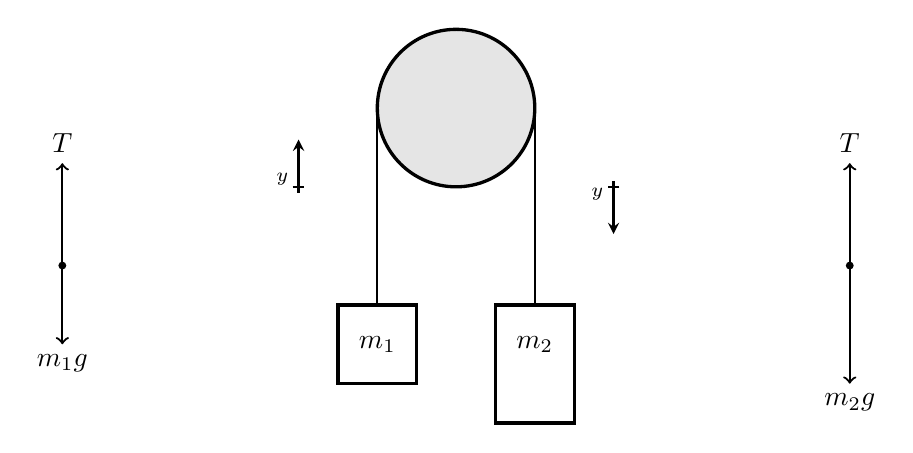
\begin{tikzpicture}[scale=1]
     	
	
	
\begin{scope}[shift={(0,0)}, scale=1]
	\fill[color=gray!20] (0,0) circle (1cm);
	\draw[very thick] (0,0) circle (1cm);
	\draw[thick] (1,0) -- (1,-2.5); 
	\draw[thick] (-1,0) -- (-1,-2.5); 
	\draw[very thick] (-1.5,-2.5) -- (-0.5,-2.5) -- (-0.5,-3.5) -- (-1.5,-3.5) -- cycle;
	\draw (-1,-3) node [anchor=center] {$m_1$};
	\draw[very thick] (1.5,-2.5) -- (0.5,-2.5) -- (0.5,-4) -- (1.5,-4) -- cycle;
	\draw (1,-3) node [anchor=center] {$m_2$};	
\end{scope}

   	  \begin{scope}[shift={(-2,-1)}, scale=0.75,rotate=0] 
	  \draw[ thick,-stealth] (0,-0.1) -- (0,0.8) node [near start,anchor=east]{\scriptsize $y$};  
	  \draw[thick](-0.1,0) -- (0.1,0);
	  \end{scope}
	  
	    \begin{scope}[shift={(2,-1)}, scale=0.75,rotate=180] 
	  \draw[ thick,-stealth] (0,-0.1) -- (0,0.8) node [near start,anchor=east]{\scriptsize $y$};  
	  \draw[thick](-0.1,0) -- (0.1,0);
	  \end{scope}
	  
	  \begin{scope}[shift={(-5,-2)}, scale=1,rotate=0] 
	  \draw[->,thick] (0,0) -- (0,1.3) node [anchor=south ,scale=1] {$T$}; 
	\draw[->,thick] (0,0) -- (0,-1) node [anchor=north ,scale=1] {$m_1g $}; 
    	\fill[black] (0,0) circle (0.5mm);   
	  \end{scope}
	  
	   \begin{scope}[shift={(5,-2)}, scale=1,rotate=0] 
	  \draw[->,thick] (0,0) -- (0,1.3) node [anchor=south ,scale=1] {$T$}; 
	\draw[->,thick] (0,0) -- (0,-1.5) node [anchor=north ,scale=1] {$m_2g $}; 
    	\fill[black] (0,0) circle (0.5mm);   
	  \end{scope}
	  
	 
    
   \end{tikzpicture}
   $$
   $$\text{1:}\ \ \ \overrightarrow{F}_{1,net}=\overrightarrow{F}_{1,g}+\overrightarrow{T}_1=(\ \ T-m_1g)\hat{y}=m_1\overrightarrow{a}$$
    $$\text{2:}\ \ \ \overrightarrow{F}_{2,net}=\overrightarrow{F}_{2,g}+\overrightarrow{T}_2=(-T+m_2g)\hat{y}=m_2\overrightarrow{a}$$

$$T-m_1g=m_1a$$
$$-T+m_2g=m_2a$$

$$ a=\frac{g(m_2-m_1)}{m_1+m_2} \ \ \ \text{and} \ \ \  T=\frac{(m_1-m_2)a+(m_1+m_2)g}{2}=\frac{2gm_1m_2}{m_1+m_2}$$

\section{Circular Motion}

\marginnote[10pt]{Circular motion is best analyzed determining the components of force in the tangential and radial direction.  The net radial force functions as the centripetal force.  The tangential components of the forces change the speed of the mass. }




$$\begin{tikzpicture}[scale=1]
     	
	
	
\draw [color=gray!80] (0,0)--(3,0)
   node [midway,anchor=south,inner sep=1pt, outer sep=1pt]{$R$};


 \begin{scope}[shift={(0,0)}, scale=1,rotate=120] 
 \draw[color=gray,dashed] (0,0) circle (3cm);
  \begin{scope}[shift={(0,-4)}, scale=0.75, rotate=-90] 
	  \draw[ thick,-stealth] (0,-0.1) -- (0,0.8) node [near start,anchor=east]{\scriptsize $\theta$};  
	  \draw[thick](-0.1,0) -- (0.1,0);
	   \draw[thick](0.2,-0.4) -- (0.2,-0.6);
	    \draw[ thick,-stealth] (0.1,-0.5) -- (1,-0.5) node [near start,anchor=north]{\scriptsize $r$};  
	  \end{scope}
 \fill[black] (0,0) circle (1mm);  
 \draw [very thick] (0,0) -- (0,-3);
 \fill[color=white] (0.5,-2.5) -- (-0.5,-2.5) -- (-0.5,-3.5) -- (0.5,-3.5) -- cycle;
  \draw[very thick] (0.5,-2.5) -- (-0.5,-2.5) -- (-0.5,-3.5) -- (0.5,-3.5) -- cycle;
  \draw (0,-3) node {$m$};
 \end{scope}
		  
	   \begin{scope}[shift={(9,0)}, scale=1,rotate=120] 
	  \draw[->,thick] (0,0) -- (0,1.3) node [anchor=east ,scale=1] {$F_{c}$}; 
	   \draw[->,thick] (0,0) -- (-0.7,0) node [anchor=north ,scale=1] {$F_{t}$}; 
    	\fill[black] (0,0) circle (0.5mm);   
	  \end{scope}
	  
	    \begin{scope}[shift={(6,0)}, scale=1,rotate=120] 
	
	   \draw[->,thick] (0,0) -- (-0.7,1.3) node [anchor=north ,scale=1] {$F_{net}$}; 
    	\fill[black] (0,0) circle (0.5mm);   
	  \end{scope}
	  
	  
    
   \end{tikzpicture}$$
   $$\overrightarrow{F}_{net}=m\overrightarrow{a}=mr\ddot{\theta}\hat{\theta}-m r\dot{\theta}^2\hat{r}$$
   $$F_t=mr\ddot{\theta}=mr\alpha=ma_t$$
   $$F_c=mr\omega^2=m\frac{v^2}{r}=ma_c$$
\section{Non-Inertial Frames}
\marginnote[20pt]{In a non-inertial frame a fictional force is observed in the opposite direction of the acceleration of the frame.  For example, a frame accelerated centripetally will exhibit a centrifugal pseudo-force.  The Coriolis effect is another example of pseudo-forces in action. }
$$\begin{tikzpicture}[scale=1]
     	
	 \draw[color=gray,dashed] (-2,-2) -- (2,-2) -- (2,2) -- (-2,2) -- cycle;
	  \draw [thick,->] (2,2) -- (3,1.5) node [anchor=west]{$\overrightarrow{a}_{frame}$};
	  
	

 \draw[->,thick] (0,0) -- (-1,0.5) node [anchor=south ,scale=1] {$\overrightarrow{F}_{pseudo}$}; 
    	\fill[black] (0,0) circle (0.5mm);   


	  \draw (6,0) node {$\overrightarrow{F}_{pseudo}=-m\overrightarrow{a}_{frame}$};
	  
    
   \end{tikzpicture}$$
   



\section{Accelerometers}
$$\begin{tikzpicture}[scale=1]
     	
	 \draw[color=gray,dashed] (-2,-2) -- (2,-2) -- (2,2) -- (-2,2) -- cycle;
	  \draw [thick,->] (2,2) -- (3,1.5) node [anchor=west]{$\overrightarrow{a}_{frame}$};
	  
	
\draw[->,thick] (0,0) -- (0,-1) node [anchor=north,scale=1] {$\overrightarrow{F}_{g}$}; 
 \draw[->,thick] (0,0) -- (-1,0.5) node [anchor=south ,scale=1] {$\overrightarrow{F}_{pseudo}$}; 
    	\fill[black] (0,0) circle (0.5mm);   


\draw (6,0) node {$\overrightarrow{F}_{accel}=\overrightarrow{F}_{pseudo}+\overrightarrow{F}_{g}$};
	  
    
   \end{tikzpicture}$$
   



\section{Universal Gravitational Force}
\marginnote[0pt]{Newton's law of universal gravitation states that any two bodies in the universe attract each other with a force that is directly proportional to the product of their masses and inversely proportional to the square of the distance between them.}

$$F_g=\frac{Gm_1m_2}{r^2} \hspace{1cm} G=6.674\times10^{-11} \frac{\text{N}\cdot\text{m}^2}{\text{kg}^2}$$
$${\overrightarrow{F}_{g}}_{1\rightarrow 2}=-\frac{Gm_1m_2}{r^2}\hat{r}=-{\overrightarrow{F}_{g}}_{2\rightarrow 1}$$


$$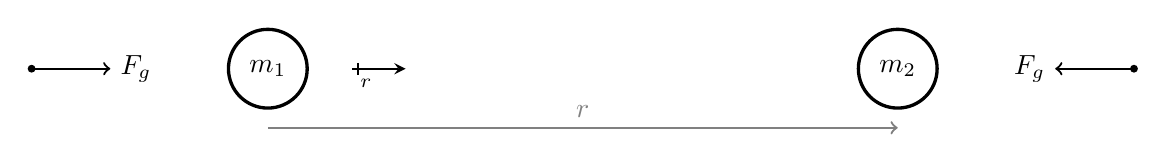
\begin{tikzpicture}[scale=1]
     	
	\fill[black] (-7,0) circle (0.5mm);   
	\draw[->,thick] (-7,0) -- (-6,0) node [anchor=west ,scale=1] {$F_g$}; 
	\fill[black] (7,0) circle (0.5mm);   
	\draw[->,thick] (7,0) -- (6,0) node [anchor=east ,scale=1] {$F_g$}; 
	 \draw[very thick] (-4,0) circle (0.5cm) node {$m_1$};
	  \draw[very thick] (4,0) circle (0.5cm) node {$m_2$};
	    \draw[thick, color=gray,->] (-4,-0.75) --   (4,-0.75) node [midway, anchor=south] {$r$};
	     
	     
	       \begin{scope}[shift={(-3,0)}, scale=0.75] 
	 
	   \draw[thick](0.2,0.1) -- (0.2,-0.1);
	    \draw[ thick,-stealth] (0.1,0) -- (1,0) node [near start,anchor=north]{\scriptsize $r$};  
	  \end{scope}
   
	     
   \end{tikzpicture}$$


\section{Spring Force}
\marginnote[0pt]{Hooke's law states that the force needed to extend or compress a spring by some distance is directly proportional to that distance.  The proportionality constant, $k$, is known as the spring constant.  The law is named after 17th century British physicist Robert Hooke. Hooke's equation in fact holds (to some extent) in many other situations where an elastic body is deformed, such as wind blowing on a tall building, a musician plucking a string of a guitar, or the filling of a party balloon. An elastic body or material for which this equation can be assumed is said to be linear-elastic or Hookean.}


$$\overrightarrow{F}_k=-k\overrightarrow{x}$$
$$\overrightarrow{F}_{net}=\overrightarrow{F}_k= -kx\hat{x}=m\overrightarrow{a}$$

\tikzstyle{spring}=[thick,decorate,decoration={zigzag,pre length=0.1cm,post
  length=0.1cm,segment length=6}]
  
  $$\begin{tikzpicture}[scale=1]
     	
	\draw[->,thick] (0,0) -- (0,1) node [anchor=south ,scale=1] {$F_k$}; 
	
	
    	\fill[black] (0,0) circle (0.5mm);   
	
	
	
	
	  \begin{scope}[shift={(-5,-1)}, scale=0.5]
	 \draw[dashed, color=gray] (-3,3) -- (3,3) node [near start, anchor =south east] {\tiny equilibrium};
	 	\draw[spring] (0,1) -- (0,5);
		 \draw[->,thick, color=gray] (2,3) -- (2,0) node [midway, anchor =west] {\small$\overrightarrow{x}$};
	  \fill[color=gray!30, path fading=north] (-3,5) -- (3,5) -- (3,7) -- (-3,7) ;
	  \draw[very thick] (-3,5) -- (3,5);  
	      	\draw[very thick] (-1,-1) -- (-1,1) -- (1,1) -- (1,-1) -- cycle;  
	 
	\draw (0,0) node [anchor=center]{$m$};
   	
   \end{scope}
   
   
   	  \begin{scope}[shift={(-2,0.2)}, scale=0.75, rotate=180] 
	  \draw[ thick,-stealth] (0,-0.1) -- (0,0.8) node [near start,anchor=east]{\scriptsize $x$};  
	  \draw[thick](-0.1,0) -- (0.1,0);  
	  \end{scope}
   \end{tikzpicture}
   $$
  
\section{Time Dependent Forces}
$$\overrightarrow{F}=\overrightarrow{F}(t)$$
\begin{itemize}
  \item Propulsion, Wind, Tide, etc
\end{itemize}

\marginnote{
  
\includegraphics[width=\linewidth]{special-forces.jpg}}


\section{Space Dependent Forces}
$$\overrightarrow{F}=\overrightarrow{F}(\overrightarrow{\scriptr})$$
\begin{itemize}
  \item Spring, Universal Gravity, Electromagnetic Forces, etc
\end{itemize}
\section{Velocity Dependent Forces}
$$\overrightarrow{F}=\overrightarrow{F}(\overrightarrow{v})$$
\begin{itemize}
  \item Drag, Magnetic Force, etc
\end{itemize}
